\section{Цель работы}
Цель данной работы заключается в освоении технологии OFDM (Orthogonal Frequency Division Multiplexing), или мультиплексирование с ортогональным частотным разделением каналов, используя программный комплекс GNU Radio.

OFDM представляет собой метод модуляции, который использует множество несущих частот. В этой схеме частотный диапазон разделяется на ряд более мелких поддиапазонов, каждый из которых модулируется отдельно. Для реализации данного типа модуляции применяется обратное быстрое преобразование Фурье.

\section{Структура устройства}
Для начала разработаем блок-схему OFDM. Представление схемы приведено ниже:
\begin{figure}[H]
    \centering
    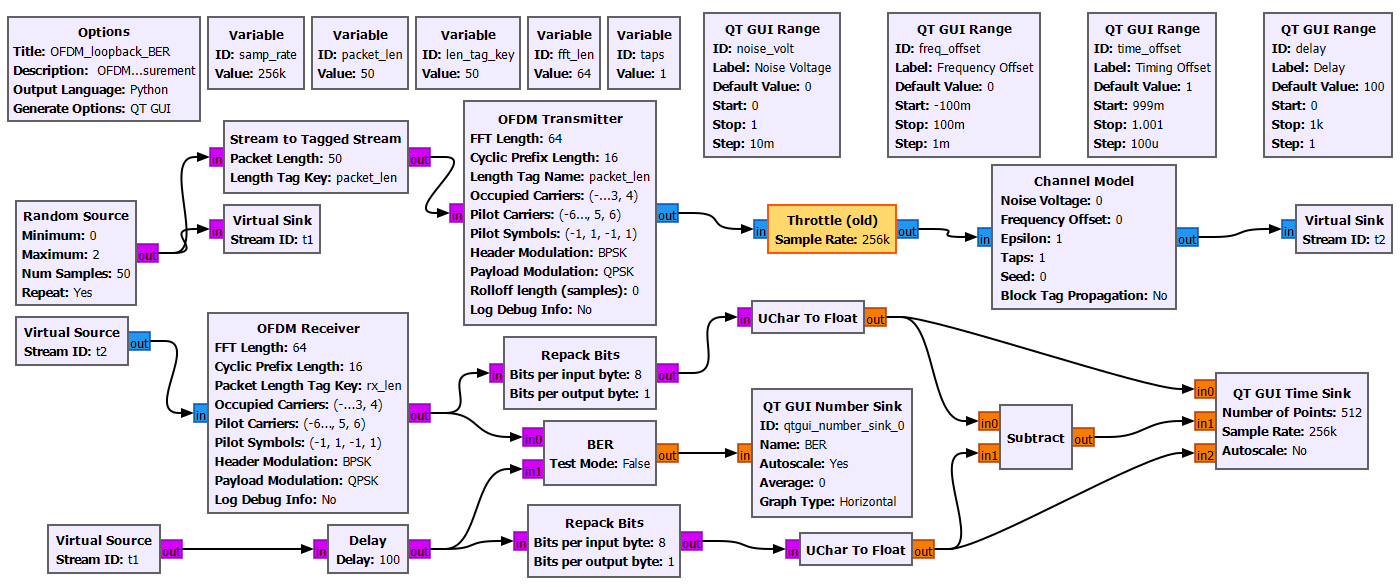
\includegraphics[width=1.0\linewidth]{Image1.png}
    \caption{Блок-схема OFDM}
    \label{fig:OFDM-schema}
\end{figure}

\section{Особенности OFDM в GNU Radio}
GNU Radio предоставляет генеричные блоки для передачи и приема OFDM-модулированных сигналов, позволяя пользователям достигать желаемой функциональности через корректную параметризацию блоков или включение собственных блоков. Добавление новой функциональности возможно с минимальными усилиями благодаря продуманному дизайну компонентов OFDM.

\subsection{FFT Shifting и Carrier Indexing}
В OFDM обычно используется FFT-сдвиг, чтобы центральная несущая была расположена в середине спектра. Индексация несущих начинается с центральной частоты и идет в обе стороны. Это обеспечивает удобство использования в различных блоках GNU Radio и поддерживает консистентность данных.

\subsection{Carrier and Symbol Allocation}
В GNU Radio блоки требуют знания о распределении несущих и символов. Это распределение регулируется объектами occupied\_carriers и pilot\_carriers для данных и пилотных символов соответственно.

\section{Испытание}
После запуска нашей системы мы наблюдаем следующий результат:
\begin{figure}[H]
    \centering
    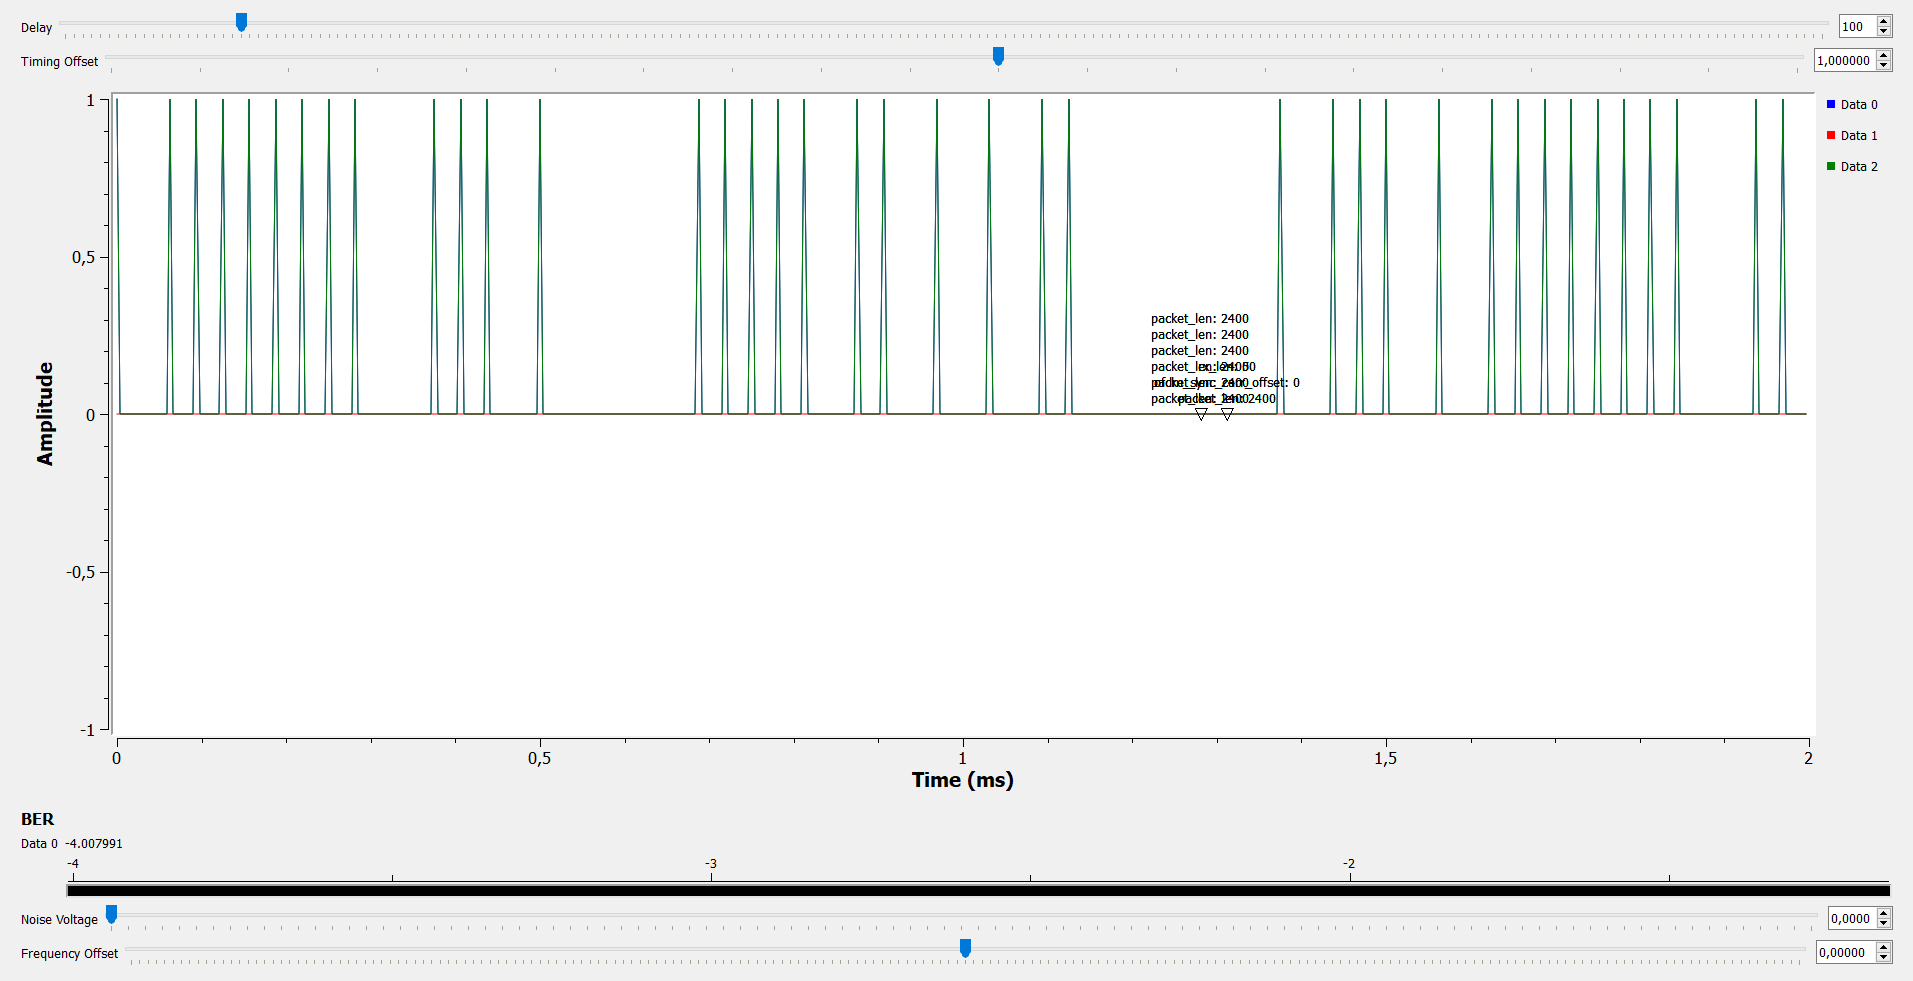
\includegraphics[width=1.0\linewidth]{Image2.png}
    \caption{Изменение амплитуды сигнала со временем}
    \label{fig:signal-amplitude}
\end{figure}
\begin{figure}[H]
    \centering
    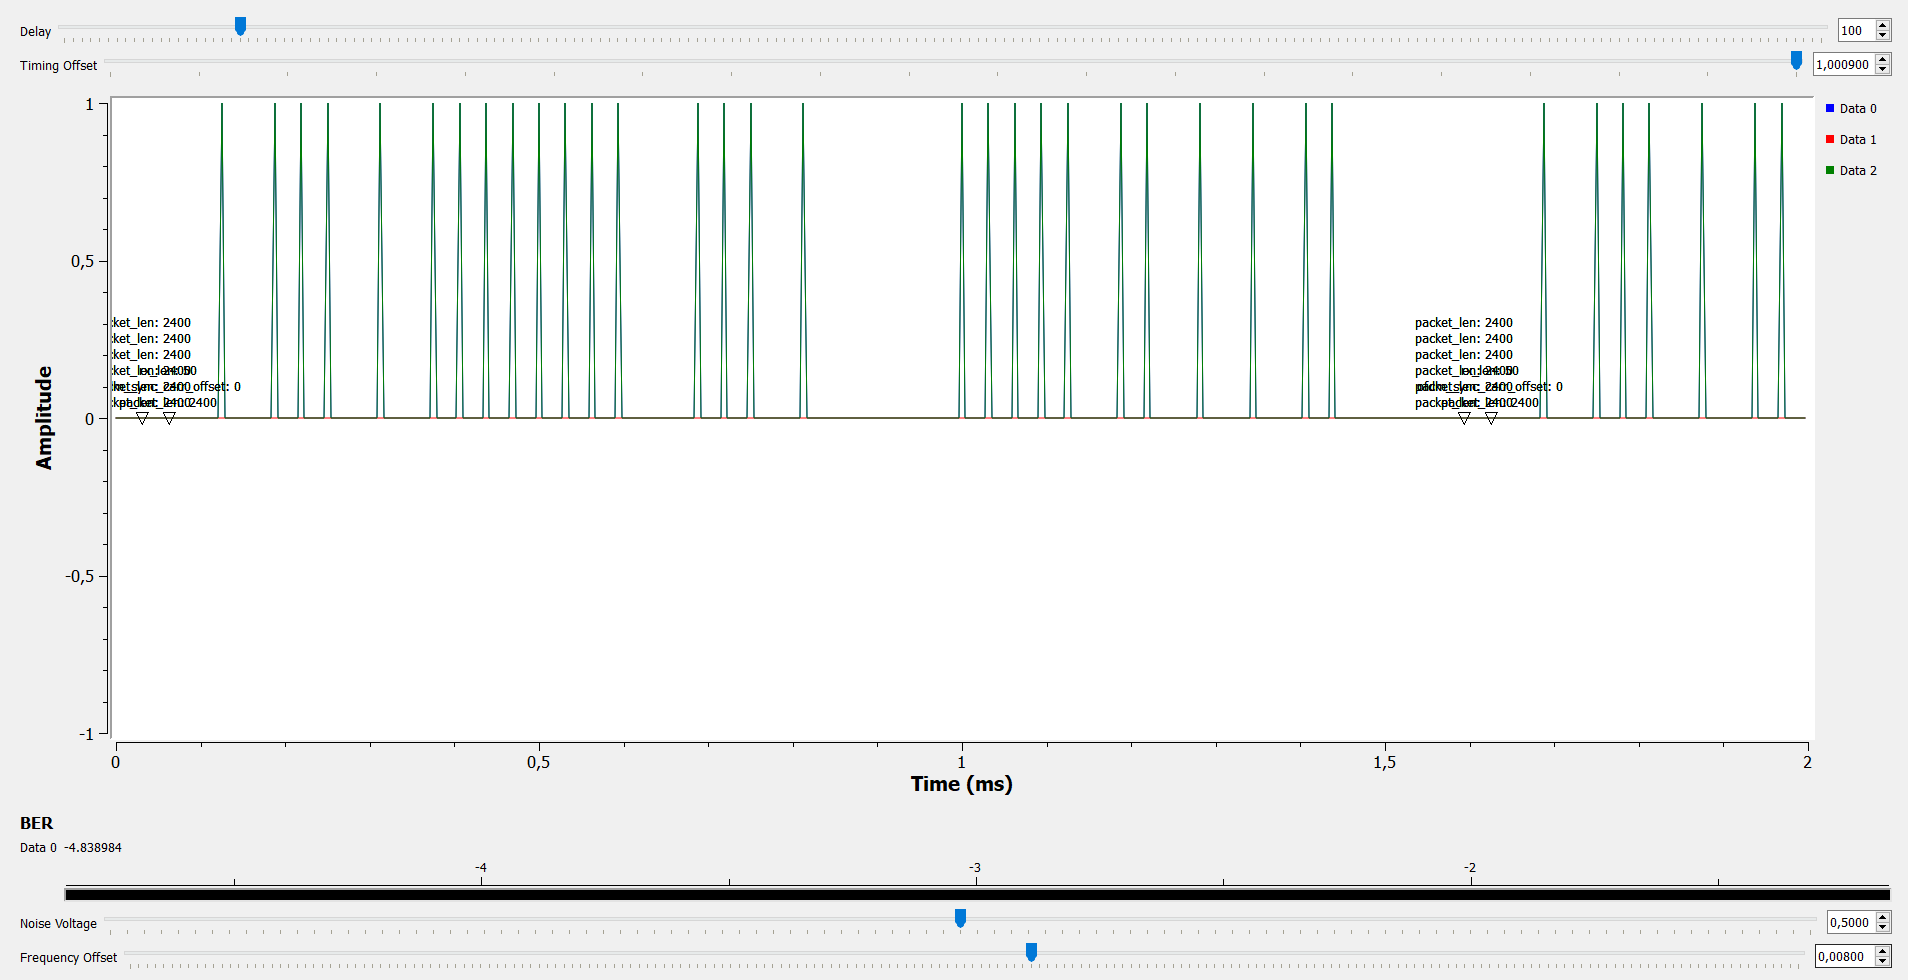
\includegraphics[width=1.0\linewidth]{Image3.png}
    \caption{Изменение амплитуды сигнала со временем}
    \label{fig:signal-amplitude2}
\end{figure}
\begin{figure}[H]
    \centering
    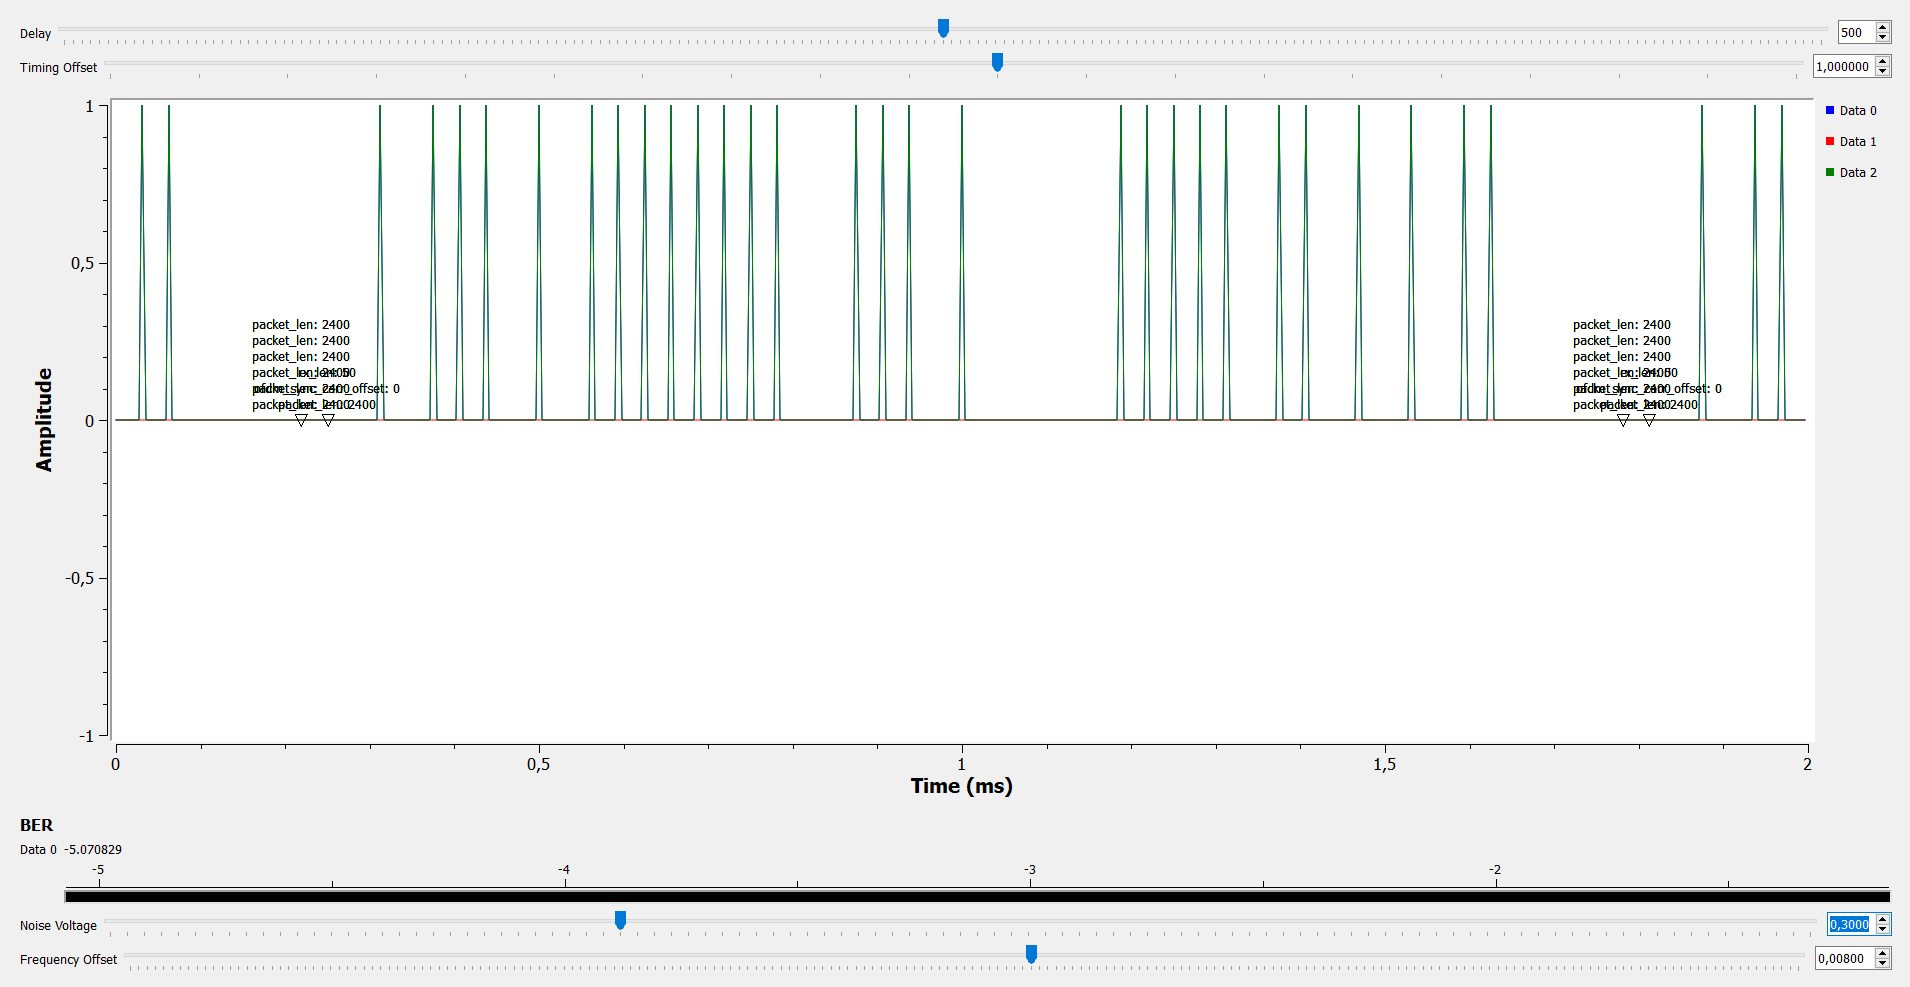
\includegraphics[width=1.0\linewidth]{Image4.png}
    \caption{Изменение амплитуды сигнала со временем}
    \label{fig:signal-amplitude3}
\end{figure}
\begin{figure}[H]
    \centering
    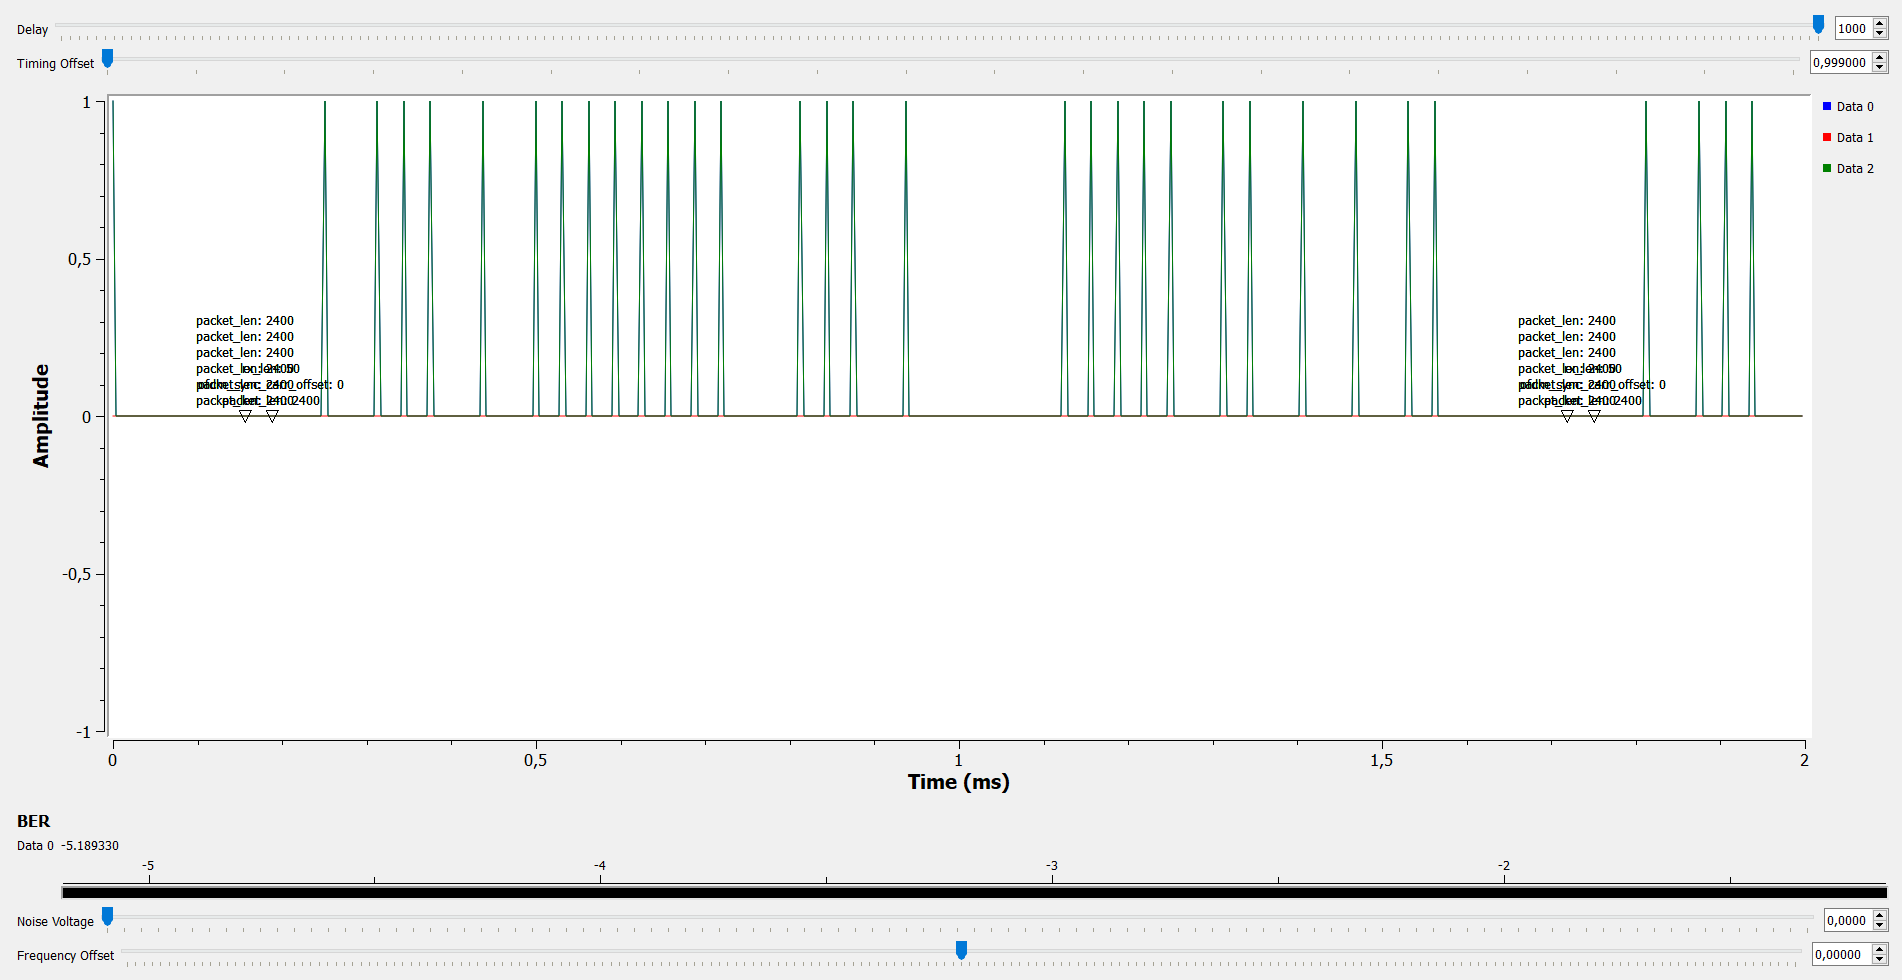
\includegraphics[width=1.0\linewidth]{Image5.png}
    \caption{Изменение амплитуды сигнала со временем}
    \label{fig:signal-amplitude4}
\end{figure}

\section{Вывод}
В процессе выполнения этой лабораторной работы были освоены практические навыки использования технологии передачи данных OFDM через GNU Radio. Важно подчеркнуть, что эта технология обладает высокой помехоустойчивостью благодаря многолучевому распространению, что позволяет проводить демодуляцию и исправление ошибок без применения сложного эквалайзера. OFDM активно применяется в промышленности, особенно в сетях 5G.